\documentclass[]{article}
\usepackage{graphicx}
\usepackage{rotating}
\usepackage{apacite}
\usepackage[numbib]{tocbibind}
\usepackage{float}

%opening
\title{Maximum entropy and population heterogeneity in 
	continuous cell cultures meet experimental data, preliminary results}
\author{}

\begin{document}
	
	\maketitle
	
	\section{Materials and Method}
	
	
	\subsection{Model framework }
	The model framework used in this work is detaily explained in \shortcite{fernandez-de-cossio-diaz_characterizing_2017} and \shortcite{fernandez-de-cossio-diaz_maximum_2019}.
	
	\subsection{Chemostat experimental data} 
	
	\subsubsection{Escherichia coli KJ134} 
	Continuous cultivation data for Escherichia coli ($E. coli$) were taken from \shortcite{van_heerden_continuous_2013}. The used Escherichia coli KJ134 strain was genetically modified for succinic acid fermentation. A dozen of steady states were recorded at different dilution rates and $GLC$ availability in the feed medium. Data for the effluent concentration of $GLC$, succinic acid ($SA$), acetic acid ($AcA$), form acid ($FA$) and malic acid ($MA$) for the different steady states were given. Also, the cell density was reported.
	
	
	\subsubsection{Human cell line AGE1.HN.AA1} 
	Experimental data were taken from \shortcite{rath_characterisation_2017}. In this work, the author performed 6 continuous cultures of the cell line AGE1.HN.AA1. Its parental line AGE1.HN was established by the company ProBioGen (ProBioGen AG, Berlin, Germany) from a tissue sample of a human brain. The experiments were run under various conditions, differing mainly in the dilution rate ($D$) and the feed medium composition of glucose ($GLC$), glutamine ($GLN$) and galactose ($GAL/GALC$) $Table\ 2$.
	
	For each experiment, a steady-state condition was reached, (steady states were labeled $A$, $B$, $C$, $D$, $E$, $F01$), and several observables were reported. Particularly relevant for this work was the growth rate ($\mu$), $D$, the viable cell density ($Xv$) and the medium concentration ($s$) and derived uptake rate ($q$) for a set of metabolites ($GLC$, lactose ($LAC$), $GLN$, ammonium ($NH4$), $GAL$, pyruvate ($PYR$), glutamate ($GLU$), alanine ($ALA$), asparagine ($ASP$)). A unit conversion was required to make experimental data and our model compatible. For this propose the only external data needed was the cell mass density, 0.25 pgDW/ $\mu$$m^3$ \shortcite{niklas_quantitative_2011}.
	
	
	\subsection{Preparing GEMs} 
	
	\subsubsection{Escherichia coli KJ134}
	For modeling the cellular metabolism, the $E. coli$ genome-scale metabolic model ($GEM$) iJR904 \shortcite{reed_expanded_2003} (download link: $https://darwin.di.uminho.pt/models$) was modified to match with \shortcite{van_heerden_continuous_2013} data. The reported genetic modifications for the Escherichia coli KJ13 strain were included. It was also added enzymatic cost constraints in concordance with \shortcite{beg_intracellular_2007}.
	
	
	\subsubsection{Human cell line AGE1.HN.AA1}
	With the same propose of modeling, the metabolism of the human-derived cell AGE1.HN.AA1, it was used a $GEM$ from \shortcite{shlomi_genome-scale_2011}(download link: $https://www.ebi.ac.uk/biomodels/MODEL1105100000$). The GEM biomass equation was modified in agreement with the biomass composition for AGE1.HN.AA1 reported in \shortcite{niklas_metabolism_2013}. The production of $\alpha$1-antitrypsin ($A1AT$) was also considered, it was used the protein sequence, $https://www.drugbank.ca/polypeptides/P01009$, and the reported production rate for $A1AT$ \shortcite{rath_characterisation_2017} to set maintenance for the required amino acids. Additionally, an atp demand ($ATPM$) was included, taking the maintenance energy demand for mammalian cells mentioned by  \shortcite{fernandez-de-cossio-diaz_physical_2018}.
		
	
	
	\newpage
	\section{Results and Discussion} 
	
	The main objective of this work is to explore the capability of an application of the Maximum Entropy ($MaxEnt$) framework to the modeling of cellular metabolism in a continuous cultivations regime. 
	$MaxEnt$ has been used for the analysis of other biology-related problems with success. 
	It has become a useful tool when we are dealing with limited data, which actually is a common scenario in biology \shortcite{de_martino_introduction_2018}. 
	
	In particular, the framework proposed in \shortcite{fernandez-de-cossio-diaz_characterizing_2017} and \shortcite{fernandez-de-cossio-diaz_maximum_2019} allows to link effectively the macroscopic variables, commonly accessible, that defined the state of a chemostat steady-state with the underlying cellular metabolism of the cells. 
	In the former article, a more traditional approach to model the metabolism was taken. It delegates in Flux Balance Analysis ($FBA$) \shortcite{orth_what_2010} for choosing the vector of reactions fluxes assumed to be determining the current metabolic state of the cell under the cultivation conditions. This method has been heavily used in the past decades with good results and a variety of applications \shortcite{obrien_using_2015}. 
	It has the advantage of not requiring kinetic parameters from cellular metabolism.
	This is possible because $FBA$ is based in a steady-state assumption, justified in the time scale difference between regulatory (slow) and metabolic (fast) processes \shortcite{de_martino_introduction_2018}. 
	Another assumption $FBA$ makes is that the cell population in the culture is homogeneous and is optimizing a given metabolic objective.
	$FBA$ returns the vector of all reactions fluxes that optimize the objective function subject to the applied constraints \shortcite{orth_what_2010}. 
	This vector will be taken as the definition of the metabolic state for all the cells in the culture, and with it, all the predictions or analyses will be made \shortcite{fernandez-de-cossio-diaz_characterizing_2017}. 
	
	To overcome the limitation of considering culture homogeneity, a probability distribution can be defined over the set of all the possible metabolic states.
	This distribution describes how probable is to find a cell in one metabolic state.
	To infer such probability distribution in agreement with available experimental data, the $MaxEnt$ principle can be used  \shortcite{fernandez-de-cossio-diaz_maximum_2019}. 
	In this work $MaxEnt$ was apply in such a way that it returns the probability distribution that maximized the entropy and ensures the expected value of the growth rate to match with the experimentally observed.
	Now, instead of a vector of reactions fluxes that optimize an objective function, the model will return a vector containing the probability distribution for each reaction flux due to the inferred $MaxEnt$ distribution. 
	This is a major advantage with respect to the $FBA$ framework, $MaxEnt$ do not assume that the cells $"have\ a\ goal"$, an objective function, it claims to compute the bias-less probability distribution in concordance with the imposed, data-driven, constraints \shortcite{de_martino_introduction_2018}. On the other hand, the main practical problem of using the metabolic $MaxEnt$ model is that it can represent a computationally expensive task, but this problem was also addressed by \shortcite{fernandez-de-cossio-diaz_maximum_2019} using expectation propagation.
	
	
	% To download
	% [1] Experimental evidence suggests the existence of evolutionary conserved global operation principles governing microbial metabolism.
	
	\subsubsection{Escherichia coli KJ134}
	
	Because good predictive results had been made using $E\ coli$ $GEMs$ \shortcite{vazquez_macromolecular_2016}, we include this model organism in our study.
	$Figures\ 1-2$ shows the results of both, $FBA$ and $MaxEnt$ models, facing the experimental data reported in \shortcite{van_heerden_continuous_2013} for $Escherichia\ coli\ KJ134$ continuous cultures. 
	In the first figure, plots of several chemostat observables vs the cell-specific dilution rate ($\xi$) are shown. 
	The parameter $\xi$ is computed as $Xv$/$D$ and can be interpreted as the number of cells sustained in the culture per unit of medium supplied per unit time \shortcite{fernandez-de-cossio-diaz_characterizing_2017}. 
	In the second figure, the corresponding correlations are displayed.
	
	As explained in the last section, the inferred $MaxEnt$ distribution ensures that the predicted growth rate ($\mu$), more precisely its expected value, coincides with the observed value, as evidenced in the upper-right graphs $Figures\ 1-2$. 
	This extra piece of information added to the model allow us to have much better correlations with respect to the $FBA$ results, $Figure\ 2$.
	In the cases of $GLC$ and $AcA$, two important metabolites related to the energetic metabolism, the improvements are notable.
	The $FA$ correlations for the $MaxEnt$ model wasn't good, but in contrast, $FBA$ is completely blind to it.
	Also, it is possible to observe in the graphs of $\mu$ and cell density ($Xv$)  that $FBA$ really over-determinate these quantities. 
	This fact may suggest, among others, that the imposed constraints are too permissive. 
	Also, although in the case of $E.\ coli$, the hypothesis of biomass maximization made by $FBA$ is generally accepted, it could not be valid for all situations.
	As explained before, $MaxEnt$ do not make this assumption, it just ajust the model to available experimental data.


	\subsubsection{Human cell line AGE1.HN.AA1}

	A more difficult task is to model the human metabolism. 
	Human related $GEMs$ are not as mature as bacteria networks \shortcite{gu_current_2019}. 
	Anyway, we applied the methodology to experimental data extracted from \shortcite{rath_characterisation_2017}. 
	$Figures\ 3$ shows the plots of several exchange fluxes as a function of the parameter $\xi$. 
	If one sees the data correlations, $Figure\ 4$, this time the results are not as polarized as in the $E.\ coli$ section but, generally $MaxEnt$ model (right columns) predictions are closer to the experimental data than ones produced by $FBA$ model (left columns). 
	Remember again that, $MaxEnt$ distribution ensures that the model growth rate match with experimental results (second row, third pair column $Figure\ 3 - 4$).
	Remarkable are the cases of $GLN$ and $PYR$, where $MaxEnt$ really make a good job improving the predictions of $FBA$. 
	Less precise, but still better for $MaxEnt$, are the cases of $ALA$ and $LAC$.  A curious case is $NH4$, where $FBA$ results were more consistent with respect to $MaxEnt$.
	Again, $FBA$ ends up over-estimating the values of $\mu$ and $Xv$, which may suggest that the cell is not actually in a state that maximizes the biomass production rate.
	For the rest of the results, $GLC$, $GLU$, $GAL$ and $ASP$, both model shows similar predictions, only satisfactory for $GLC$. 
	Because exchange fluxes and the concentration of metabolites in the effluent are two related quantities, results showed in $Figure\ 5 - 6$ mirror the former ones.
	
	It is notable that, although both models are not using a cell-line context-specific network, which is in our opinion the more significant source of error, they were capable of capturing many of the metabolic features encode in the experimental data.
	
	\begin{figure}
		\centering
		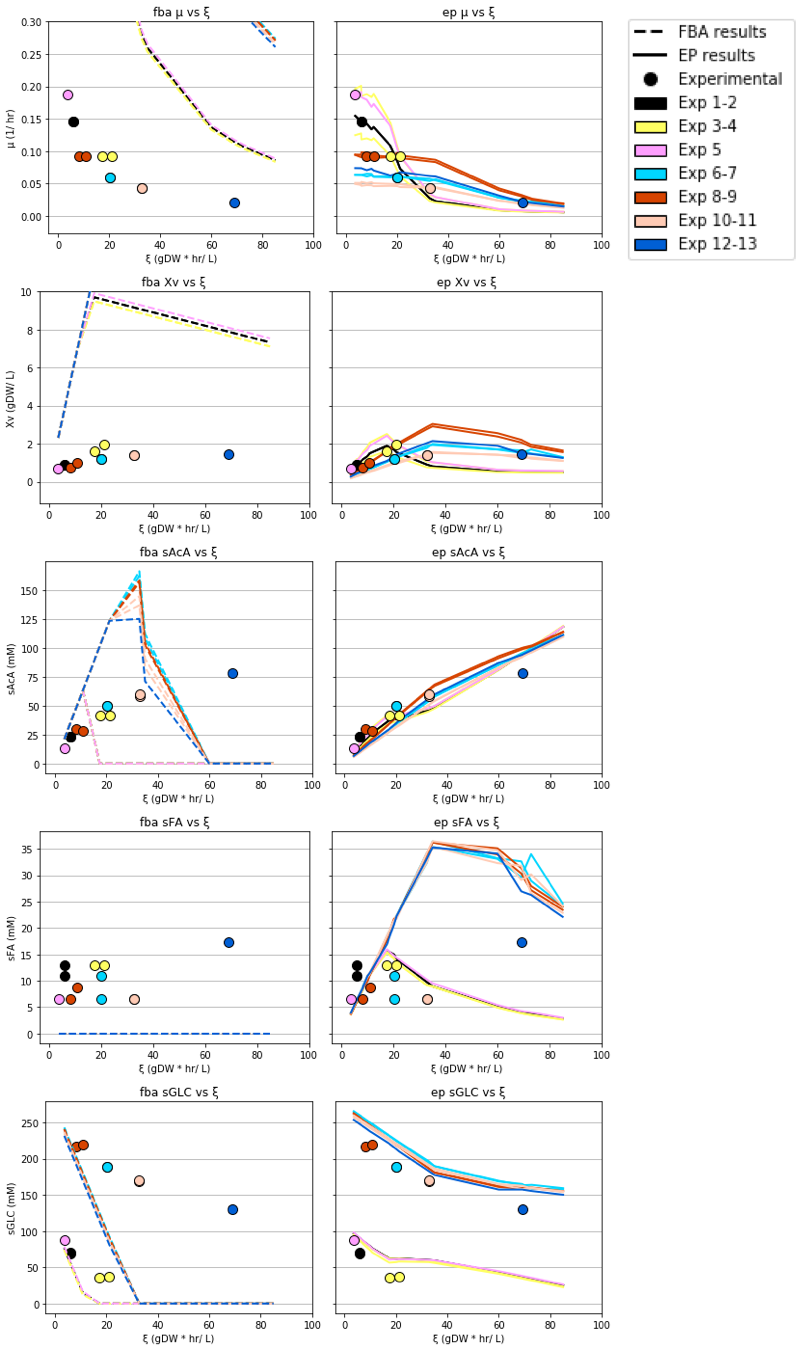
\includegraphics[scale = 0.7]{plots_s_EColi}
		\caption{Predictions (lines) of both, $FBA$ (left column) and $MaxEnt$ (right column) models, facing the experimental data (colored circles) reported in \protect\shortcite{van_heerden_continuous_2013} using $Escherichia\ coli\ KJ134$. Rows shows the growth rate ($\mu$), the cell density ($Xv$), the effluent concentration ($s$) of acetic acid ($AcA$), formic acid ($FA$) and glucose ($GLC$) respectively as a function of the cell-specific dilution rate ($\xi$) . $MaxEnt$ distribution was chosen in a manner that the expected value of the growth rate coincide with the experimental data (see first row right column)}
	\end{figure}
	
	\begin{figure}
		\centering
		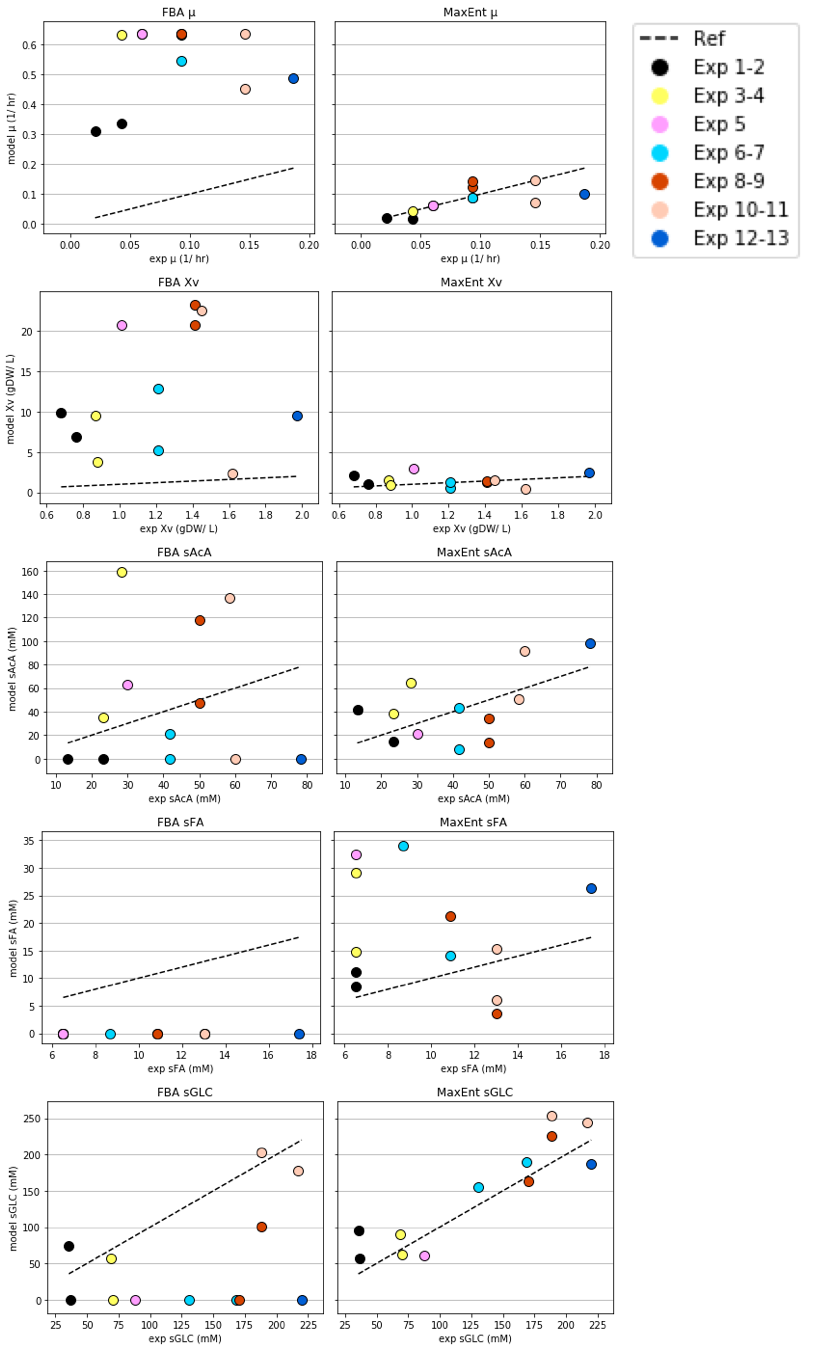
\includegraphics[scale = 0.7]{corr_s_EColi}
		\caption{Correlations of the results of both models (y axis), $FBA$ (left column) and $MaxEnt$ (right column), facing the experimental data (x axis) reported in \protect\shortcite{van_heerden_continuous_2013} using $Escherichia\ coli\ KJ134$. Rows shows the growth rate ($\mu$), the cell density ($Xv$), the effluent concentration ($s$) of acetic acid ($AcA$), formic acid ($FA$) and glucose ($GLC$) correlations respectively. $MaxEnt$ distribution was chosen in a manner that the expected value of the growth rate coincide with the experimental data (see first row right column)}
	\end{figure}
	
	\begin{sidewaysfigure}
		\centering
		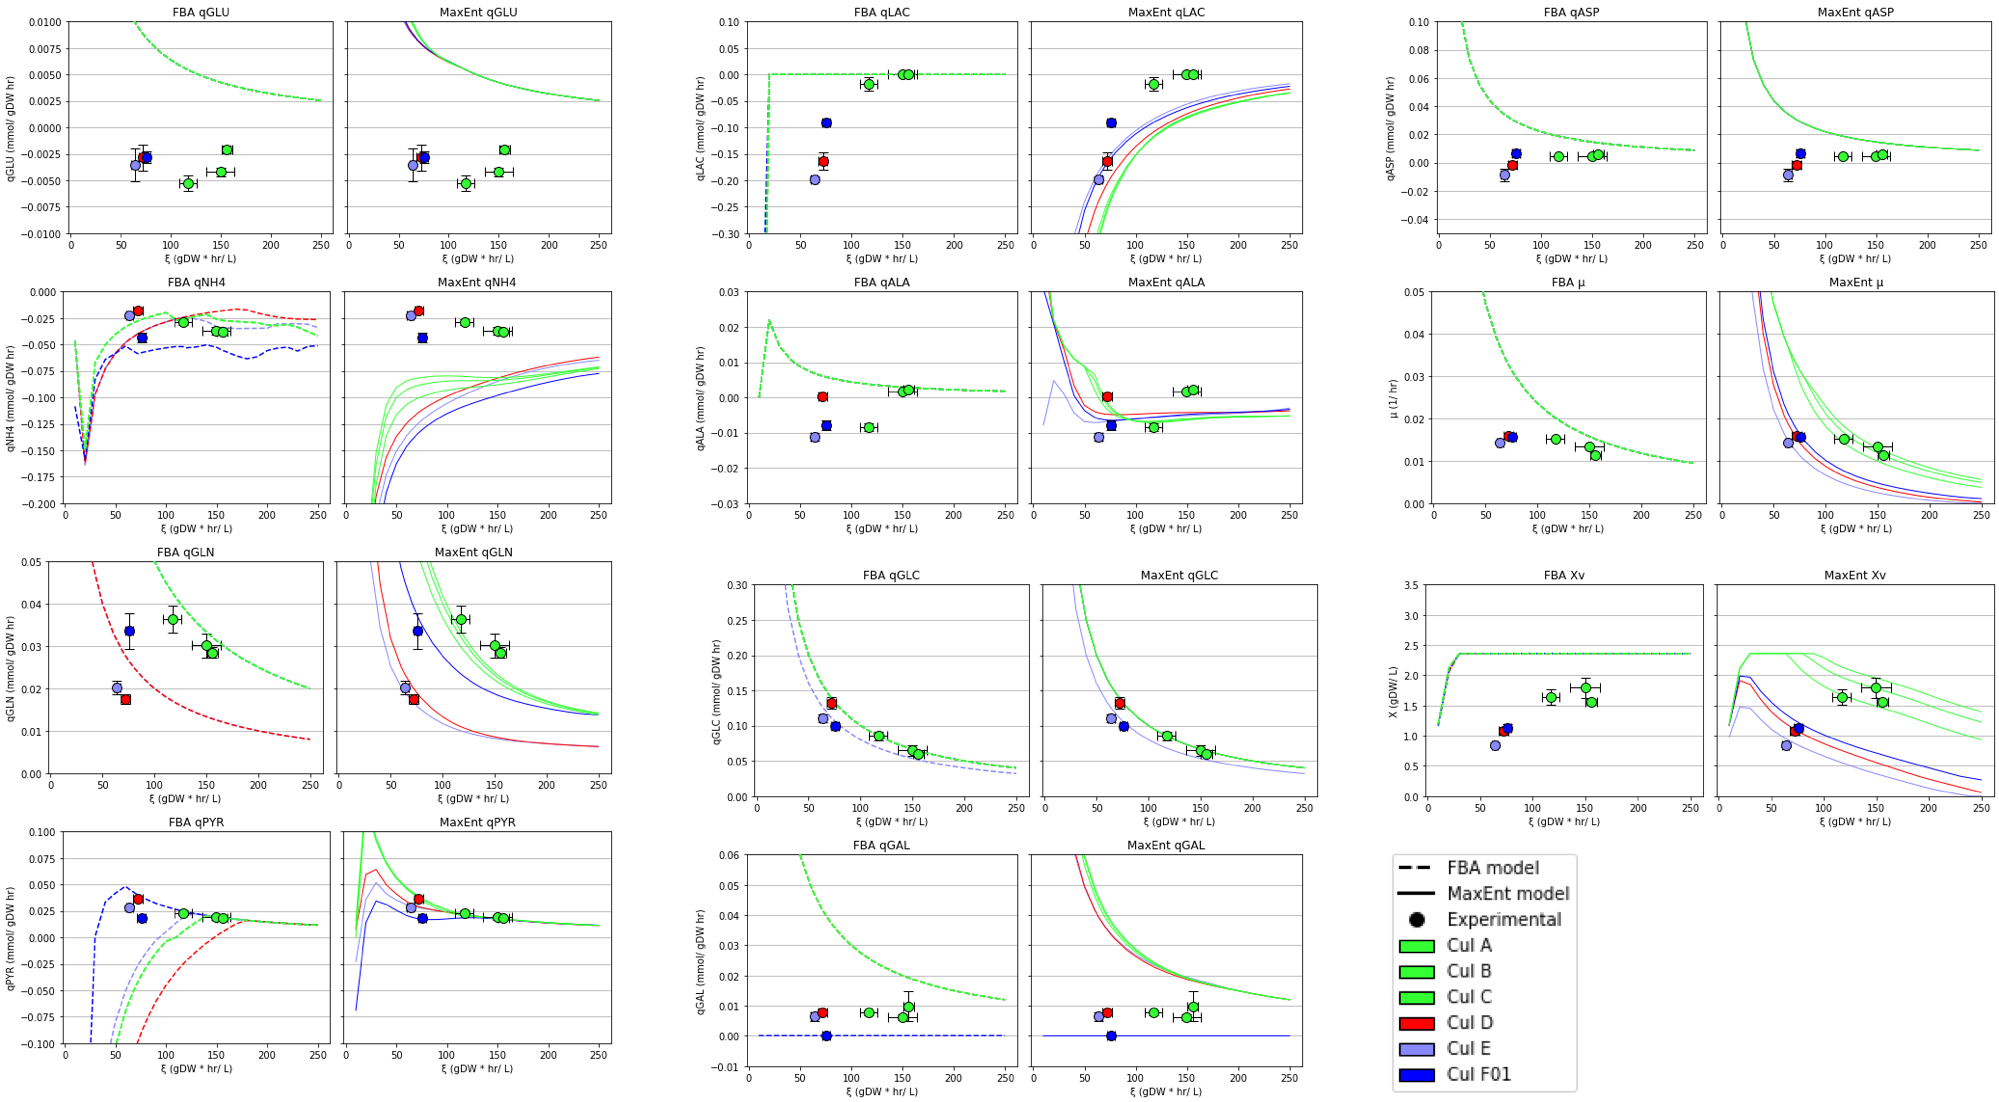
\includegraphics[scale = 0.6]{plots_q_Human}
		\caption{Exchange fluxes ($q$), growth rate ($\mu$) and cell density ($Xv$) as a function of the cell-specific dilution rate ($\xi$). Graphs are arranged as three paired columns. Each pair have the models prediction (lines),  $FBA$ (left column) and $MaxEnt$ (right column), and experimental data (colored circles) from \protect\shortcite{rath_characterisation_2017} for continuous cultures of the human derived cell line $AGE1.HN.AA1$. $MaxEnt$ distribution was chosen in a manner that the expected value of the growth rate coincide with the experimental data (see third paired colum, second row)} 
	\end{sidewaysfigure}

	\begin{sidewaysfigure}
		\centering
		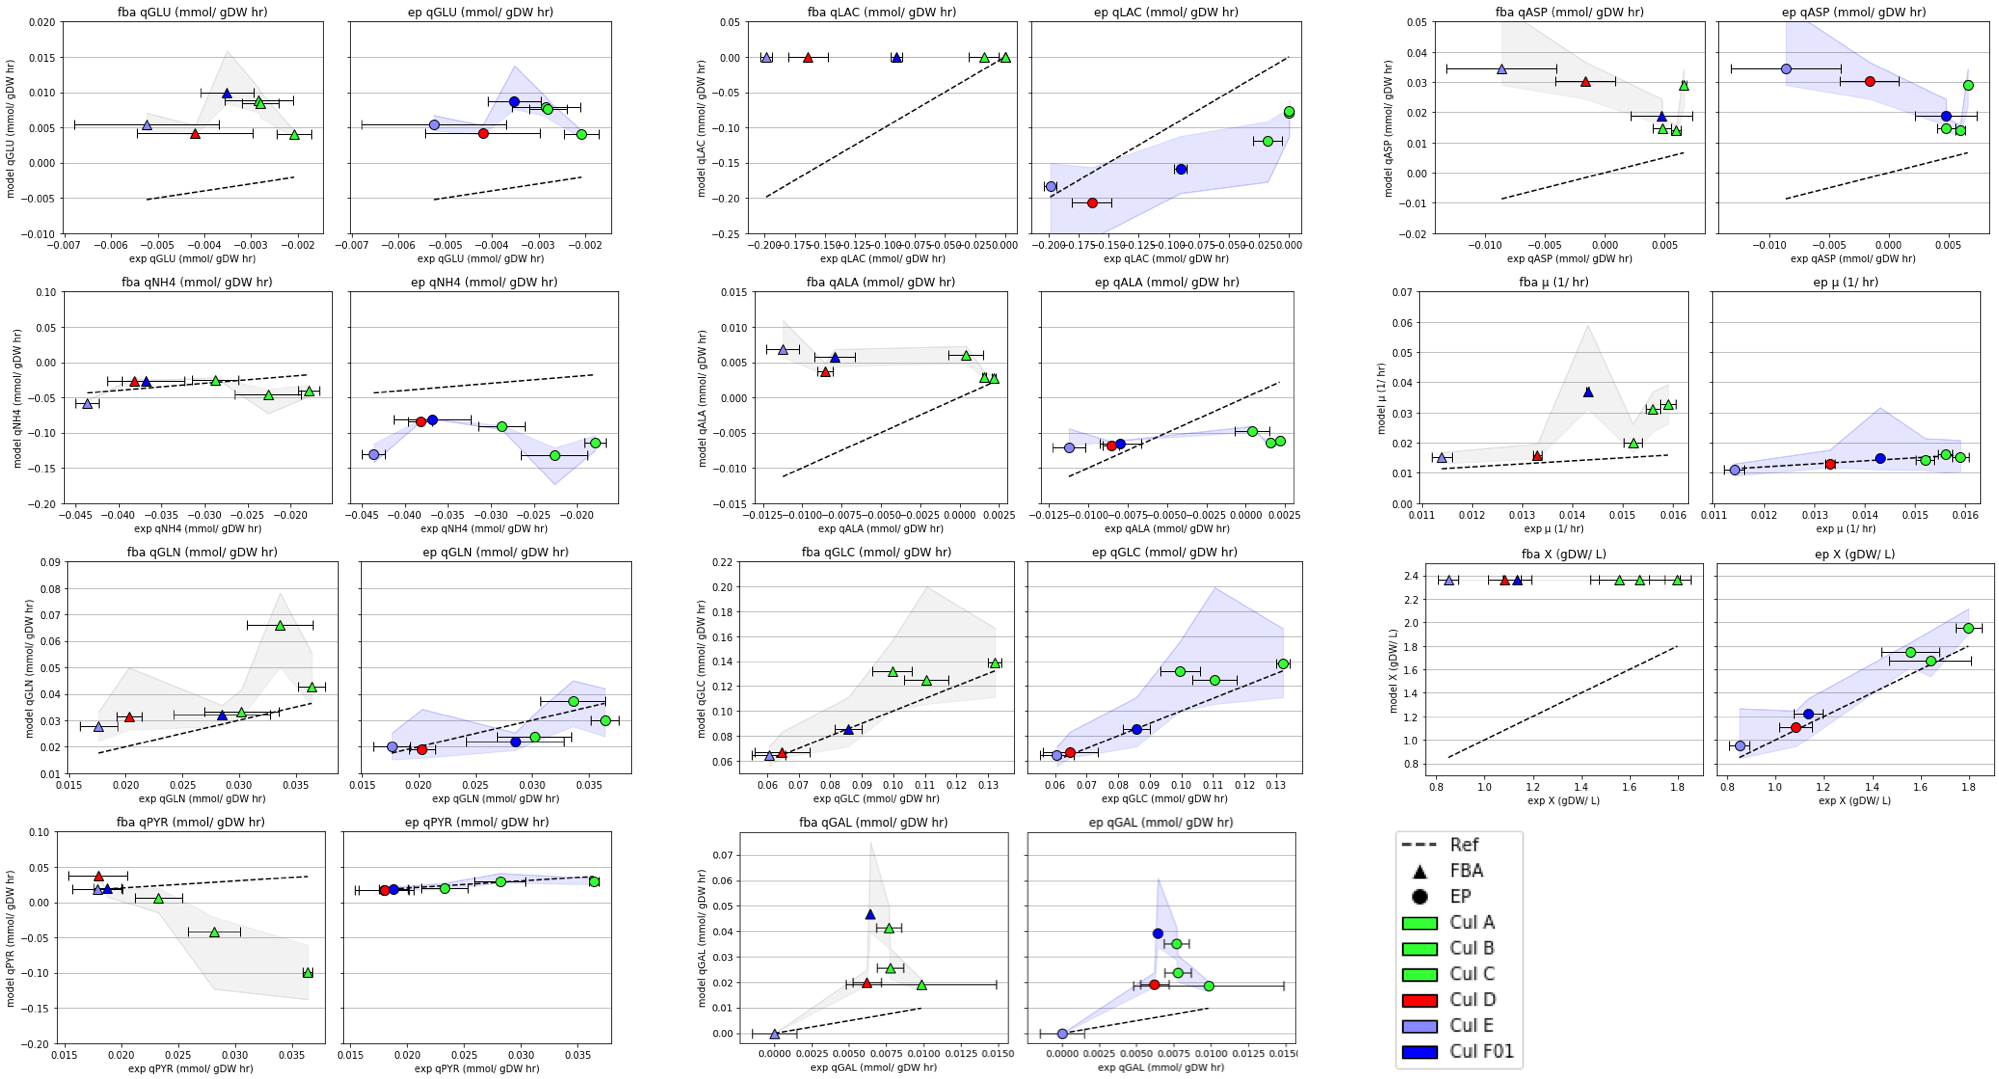
\includegraphics[scale = 0.6]{corr_q_Human}
		\caption{Correlations of the predicted (y axis) exchange fluxes ($q$), growth rate ($\mu$) and cell density ($Xv$) against experimental data (x axis) from \protect\shortcite{rath_characterisation_2017} for continuous cultures of the human derived cell line $AGE1.HN.AA1$. Graphs are arranged as three paired columns. Each pair have the correlations using $FBA$ (left column) and $MaxEnt$ (right column) models. $MaxEnt$ distribution was chosen in a manner that the expected value of the growth rate coincide with the experimental data (see third paired colum, second row)}
	\end{sidewaysfigure}

	\begin{sidewaysfigure}
		\centering
		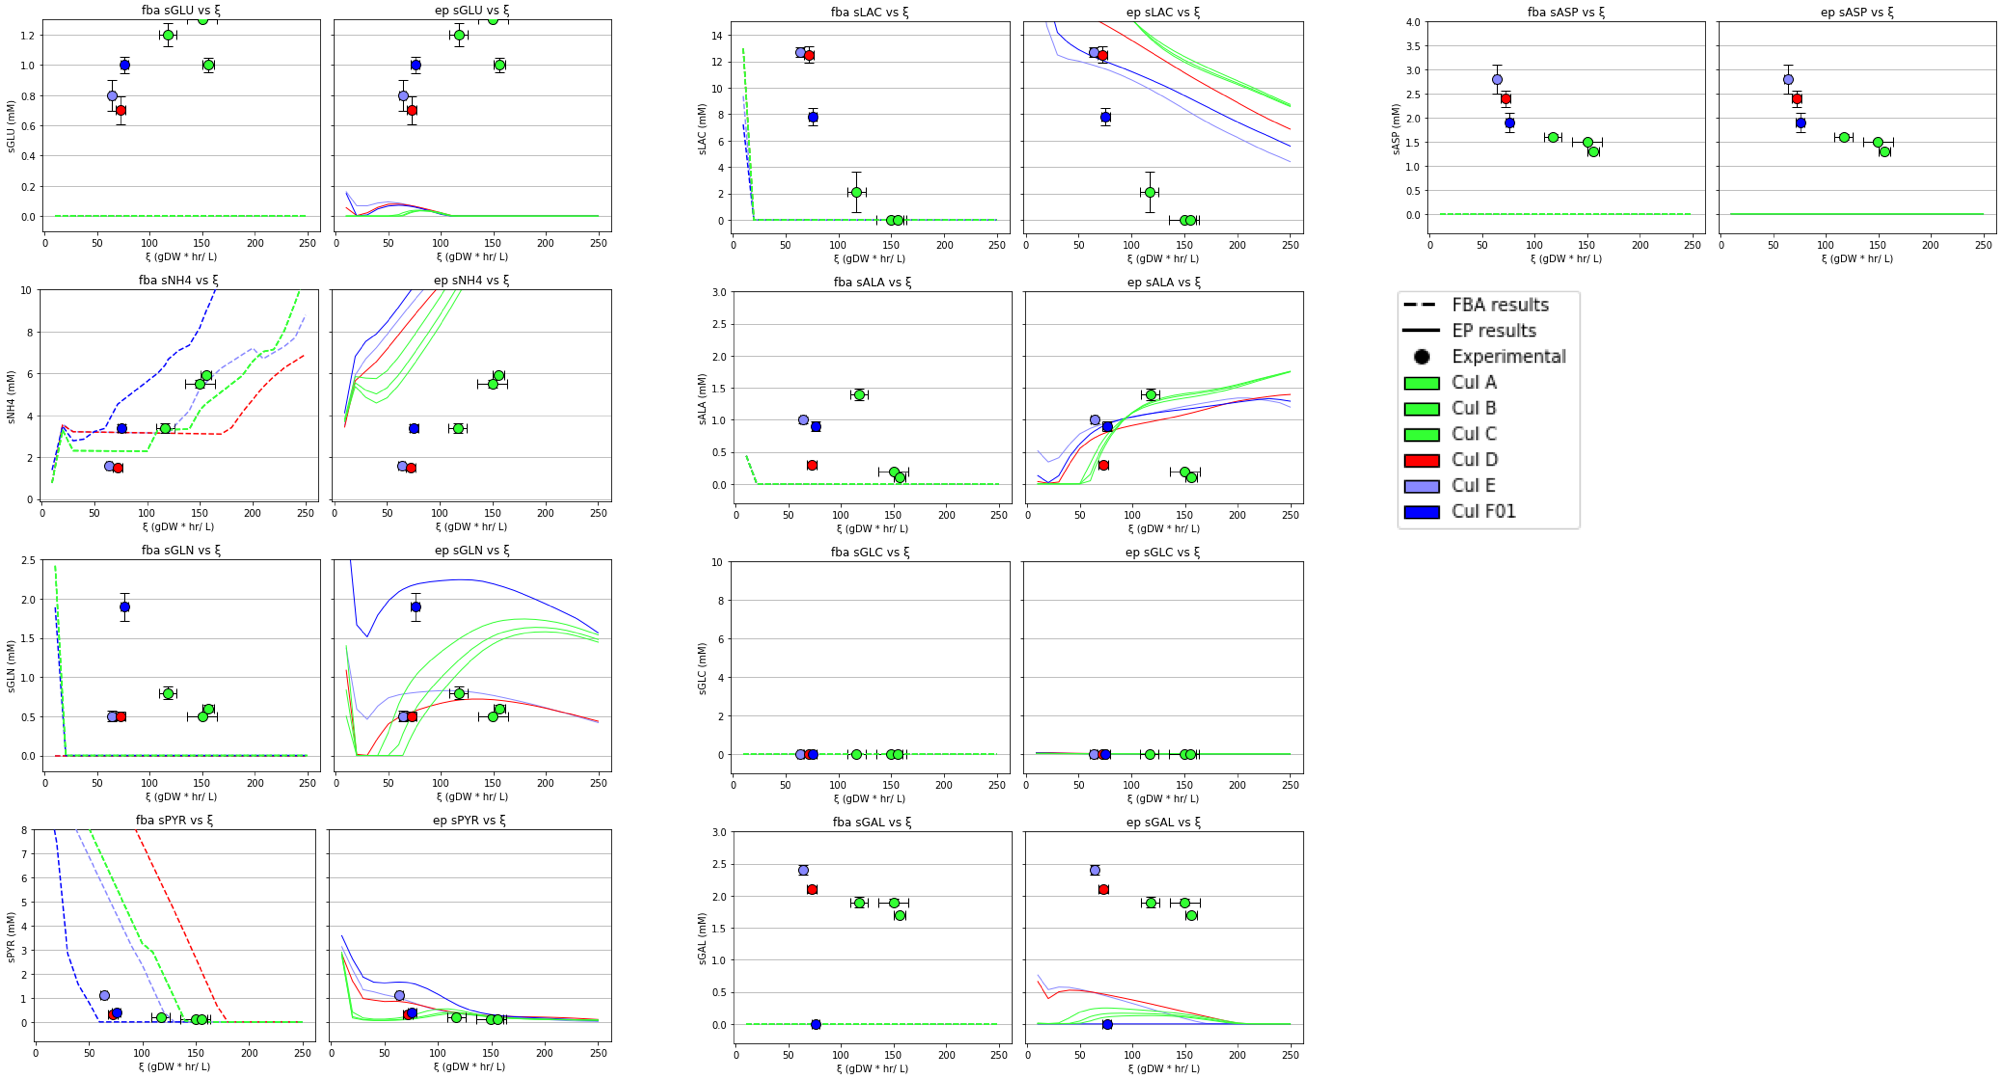
\includegraphics[scale = 0.6]{plots_s_Human}
		\caption{Metabolites effluent concentration ($s$) as a function of the cell-specific dilution rate ($\xi$). Graphs are arranged as three paired columns. Each pair have the models prediction (lines),  $FBA$ (left column) and $MaxEnt$ (right column), and experimental data (colored circles) from \protect\shortcite{rath_characterisation_2017} for continuous cultures of the human derived cell line $AGE1.HN.AA1$}
	\end{sidewaysfigure}

	\begin{sidewaysfigure}
		\centering
		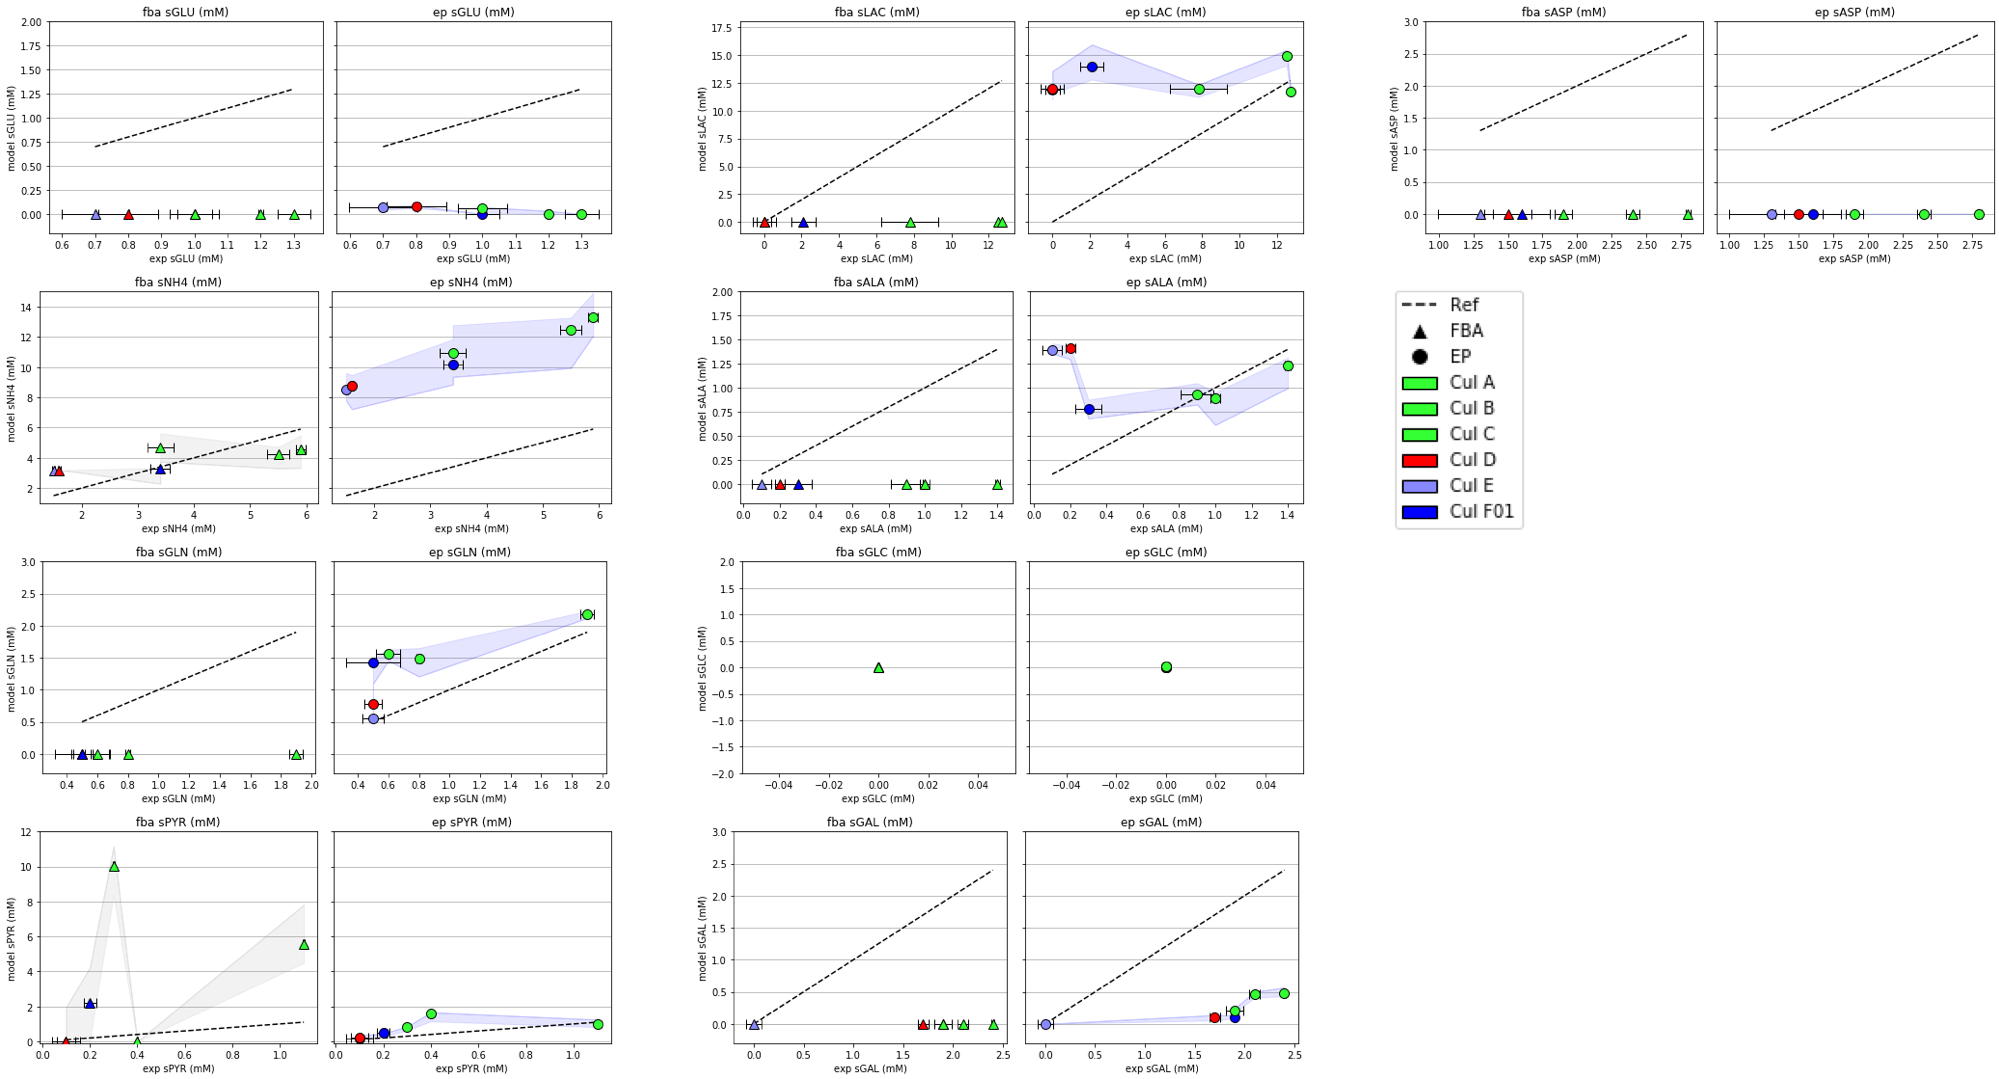
\includegraphics[scale = 0.6]{corr_s_Human}
		\caption{Correlations of the predicted (y axis) metabolites effluent concentration ($s$) against experimental data (x axis) from \protect\shortcite{rath_characterisation_2017} for continuous cultures of the human derived cell line $AGE1.HN.AA1$. Graphs are arranged as three paired columns. Each pair have the correlations using $FBA$ (left column) and $MaxEnt$ (right column) models.}
	\end{sidewaysfigure}	
	
	\newpage
	% Bibliography!!!!
	\bibliographystyle{apacite}
	\bibliography{/Users/Pereiro/Documents/zotero.bib}
	
\end{document}

